%%%%%%%%%%%%%%%%%%%%%%%%%%%%%%%%%%%%%%%%%%%%%%%%%%%%%%%%%%%%%%%%%%%%%%%%%%%%%%%
\section{Flujometrías}

De la pirmera iteración se obtuvo la geometría y datos operativos del motor, lo
cual permitió representar la curva de diferencia de presión ($\Delta P$) en
función de la alzada ($l_{v}$) de ambos puertos para diferentes velocidades de
giro, identificando los puntos de mayor interés en los cuales realizar las
flujometrías.
%
Los pares $(l_{v}, \Delta P)$ seleccionados para modelar el flujo del puerto se
detallan en las Figuras~\ref{fig:delta_p_admision} y~\ref{fig:delta_p_escape}.
%
Inicialmente se propusieron 51 flujometrías pudiendo realizar un total de 36
simulaciones que devoliveron 56 valores de $C_{D}$.

\begin{figure}[h!]
  \centering
  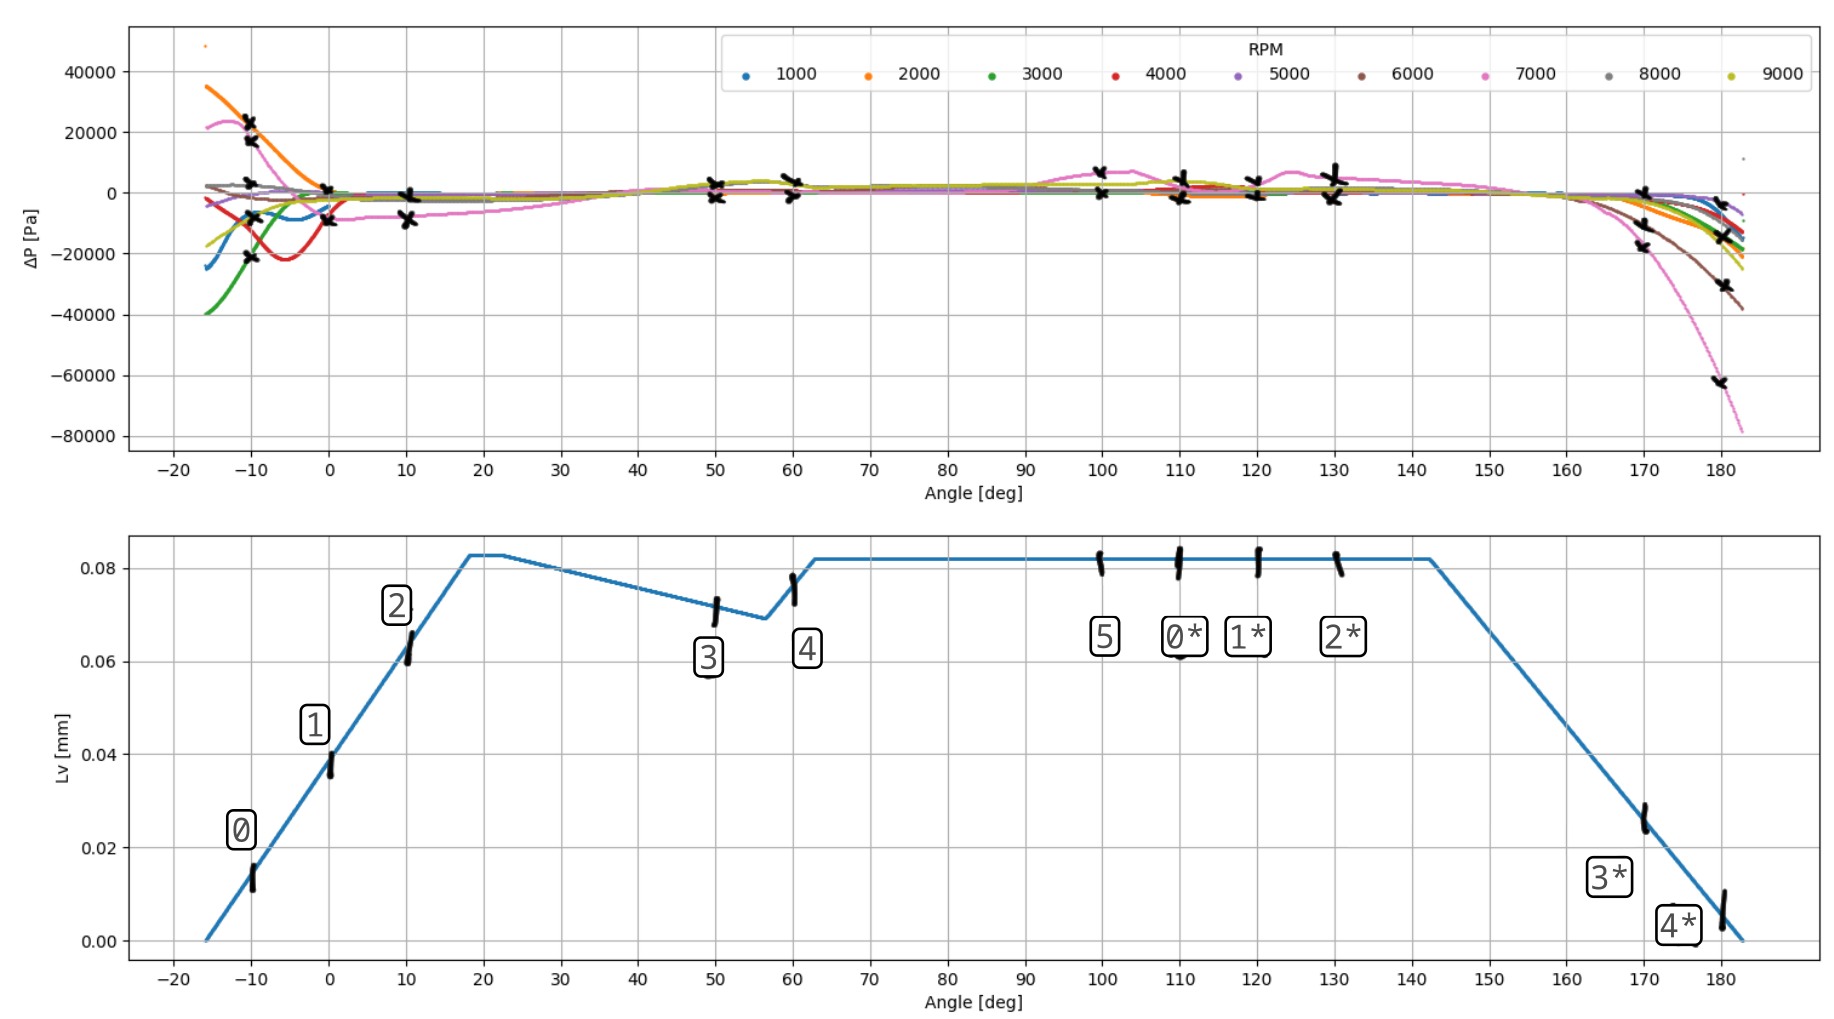
\includegraphics[width=\textwidth]{flujometrias/admision_delta_p_anot.png}
  \caption{Flujometrías puerto de admisión}\label{fig:delta_p_admision}
\end{figure}

\begin{figure}[h!]
  \centering
  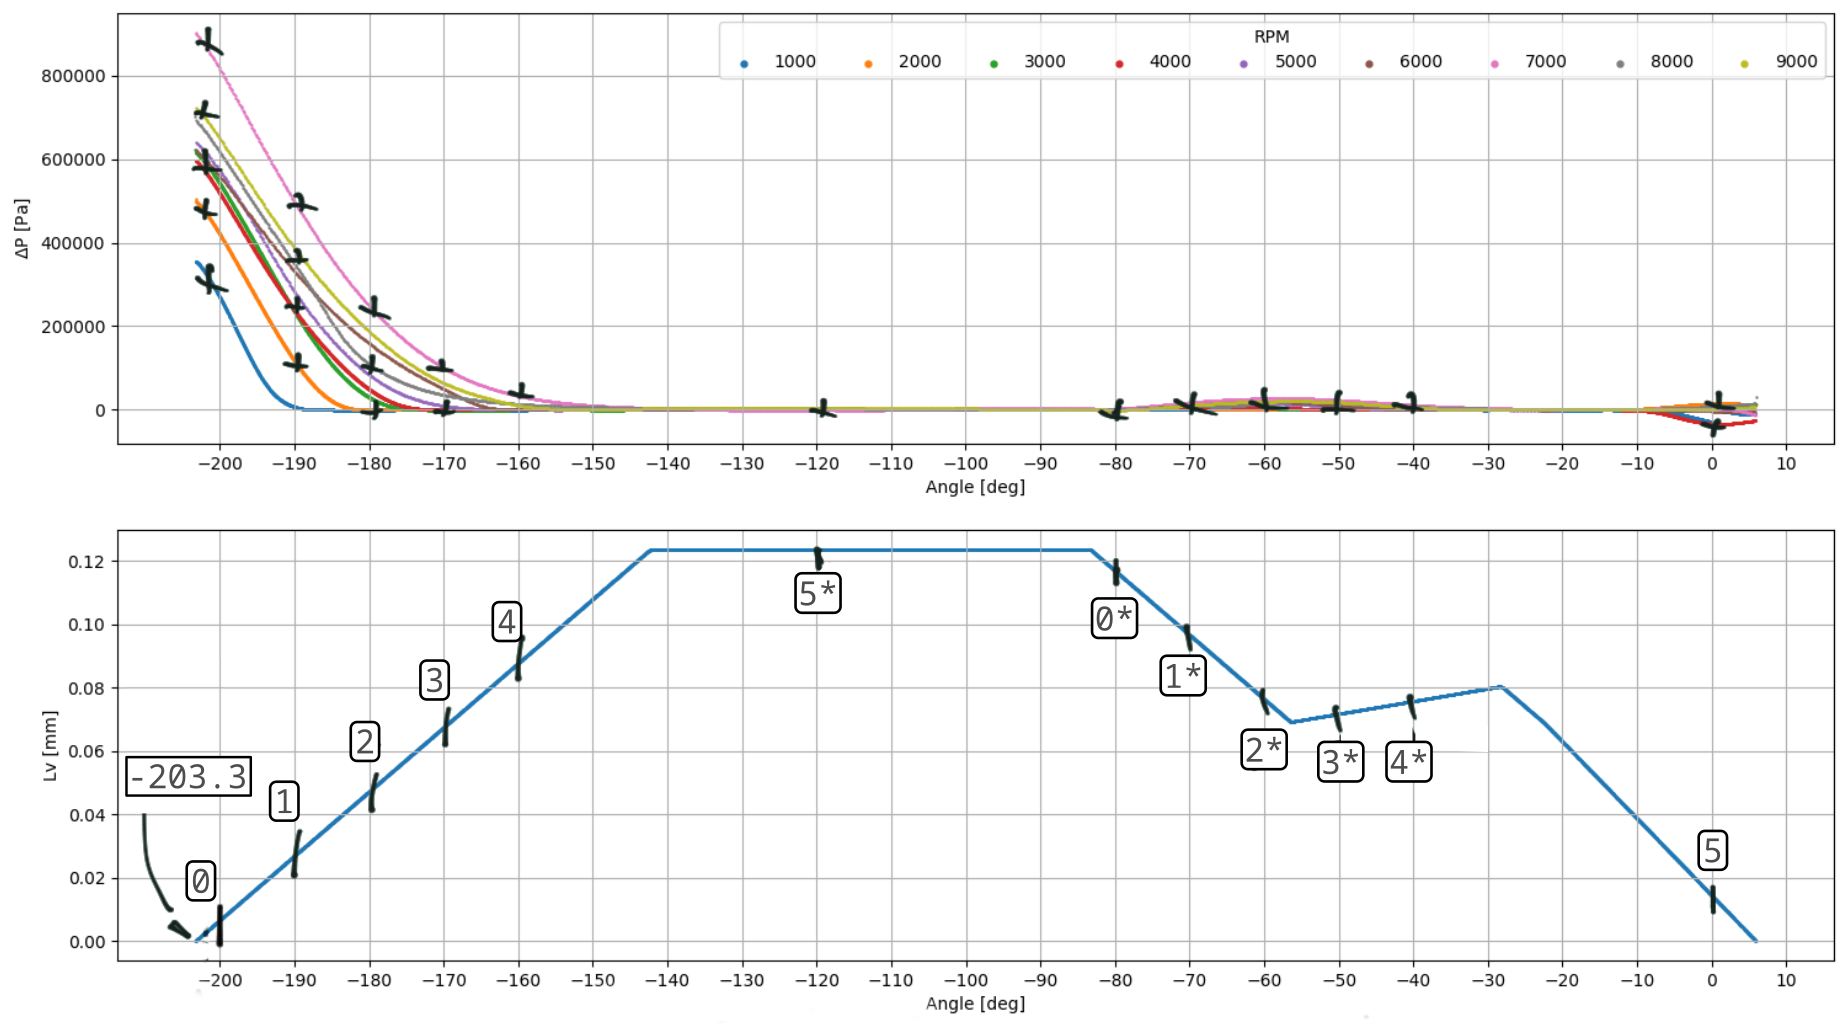
\includegraphics[width=\textwidth]{flujometrias/escape_delta_p_anot.png}
  \caption{Flujometrías puerto de escape}\label{fig:delta_p_escape}
\end{figure}


Algunas flujometrías se realizaron en tres etapas, partiendo de una malla gruesa
con celdas de $15$ mm de tamaño inicial y culminando en celdas de $5$ mm.
%
En otros se realizó directamente la flujometría con mallas base de $5$ mm.

En general se simularon alrededor de $0,02$ segundos de flujo, suficiente para
alcanzar un valor estable del caudal másico, como se ejemplifica en la
Figura~\ref{fig:adm_10_7000rpm}, donde se muestra el desarrollo de la simulación
en términos de $\dot{m}$ para el puerto de admisión con el cigüeñal en
$\theta=10^{\circ}$.
%
Para esta flujometría en particular se tiene un flujo de los gases desde la
cámara hacia el puerto de admisión, correspondiente a un puerto que abre

%
% La línea anaranjada sobre el final de la simulación representa la porción de
% datos que se seleccionó para calcular $\dot{m}$, lo cual se realizó tomando la
% media de los últimos $n$ valores obtenidos de los resultados de las flujometrías
% para los puertos de admisión y escape, las cuales se presentan en el
% Anexo~\ref{anexo:1}.
%
La totalidad de puntos evaluados se presentan en las
tablas~\ref{tab:mapa_cd_admision},~\ref{tab:mapa_cd_escape} para el puerto de
admisión y escape respectivamente.

\begin{figure}[h]
  \centering
  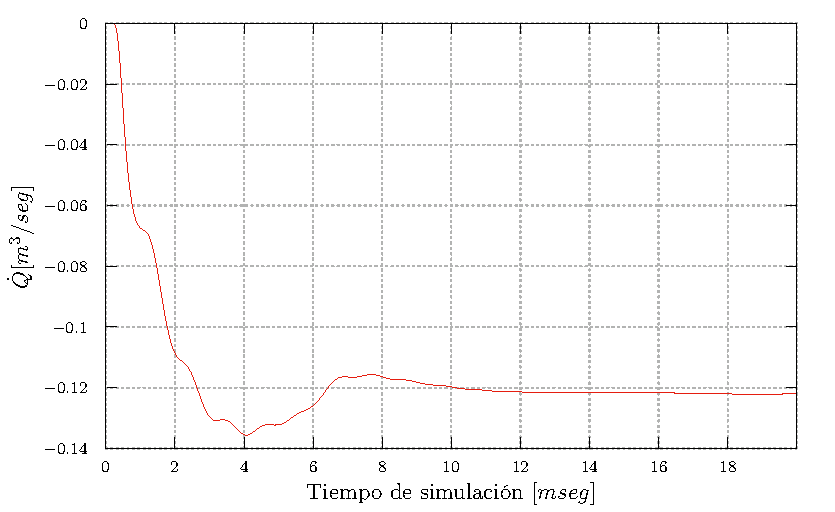
\includegraphics[]{./gnuplot/puerto_admision_10_7000.pdf}
  \caption{Puerto de admisión $10^{\circ}$ \@ $7000$ RPM}\label{fig:adm_10_7000rpm}
\end{figure}

Como se mencionó en la introducción del apartado~\ref{capitulo:DESARROLLO}, la
modificación realizada a ICESym para funcionar con un mapa de $C_{D}$
dependiente de dos variables requiere que los datos de entrada estén
distribuidos en una grilla rectangular.
%
Se utilizó entonces un método de interpolación de punto más cercano suavizado
por promedio móvil con $S=2$ para generar dicha grilla a partir de los puntos
conocidos de $C_{D}$.
%
El resultado puede observarse en las Figuras~\ref{fig:mapa_cd_admision}
y~\ref{fig:mapa_cd_escape}.
%
Con respecto al gradiente de presión indicado en las figuras que se presentan en
los párrafos siguientes, para ambos puertos se define el gradiente de presión
como la diferencia entre la presión en el cilindro y la presión en el puerto,
$\Delta P = P_{cil} - P_{puerto}$.
%
En la Tabla~\ref{tab:resumen_puertos} se resumen los valores máximos y mínimos
de $C_{D}$ y $\dot{m}$ obtenidos para los puertos de admisión y escape.

\begin{table}[h]
  \centering
  \begin{tabular}{cccccccc}\toprule
    Puerto & $l_{v} [mm]$ & $\Delta P [kPa]$ & $C_{D}$ & $\dot{m} [g/seg]$ & Nota & Figura\\ \midrule
    Admisión & 62,95 &  -7,4 & 0,59  & -122 & $C_{D,\max}$ &\ref{fig:adm_cd_max} \\
    Admisión & 81,94 &  4,95 & 0,33 &   70 & $\dot{m}_{\max}$ &\ref{fig:adm_cd_max} \\
    Escape   & 87,76 & -10,7 & 0,58 &  145 & $C_{D,\max}$ &\ref{fig:esc_cd_max}\\
    Escape   & 87,76 & -33,4 & 0,45 &  176 & $\dot{m}_{\max}$ &\ref{fig:esc_m_max}\\
  \end{tabular}
  \caption{Valores máximos y mínimos de $C_{D}$ y $\dot{m}$ para puertos}\label{tab:resumen_puertos}
\end{table}


\subsection{Puerto de Admisión}
%
En el mapa del coeficiente de descarga  para el puerto de admisión
(Fig.\ref{fig:mapa_cd_admision}) se puede observar en rojo las zonas de menor
eficiencia del escurrimiento.
%
Esto ocurre para posiciones relacionadas con la apertura y cierre del puerto
donde las presiones y velocidades de flujo involucradas son mayores aumentando
las pérdidas de carga.
%
La misma tendencia se observa si se representa el $C_{D}$ en función de la
apertura del puerto $l_{v}$ o del gradiente de presión $\Delta P$, ver
Figura~\ref{fig:cd_admision}.
%
Los mayores valores de $C_{D}$ ocurren para la mayor apertura o (en general)
para el menor gradiente de presión en términos absolutos.
%
También se observa que el coeficiente de descarga medio para el puerto es
aproximadamente 0,3.

\begin{figure}[h]
    \centering
    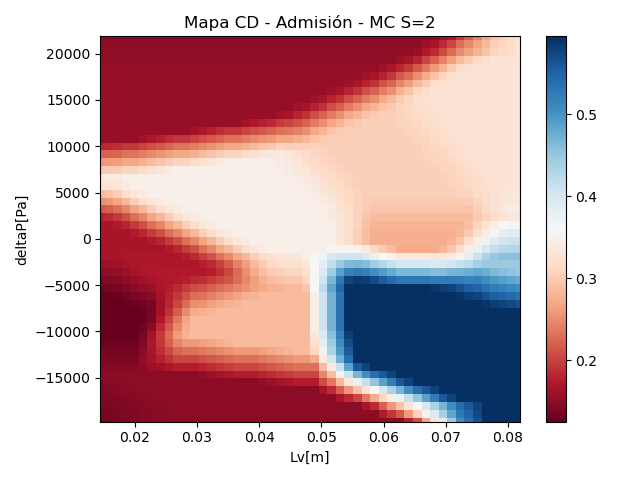
\includegraphics[width=\textwidth]{mapa_cd/mc_s2_mapa_adm.png}
    \caption{Puerto de admisión}\label{fig:mapa_cd_admision}
\end{figure}

\begin{figure}[h]
    \centering
    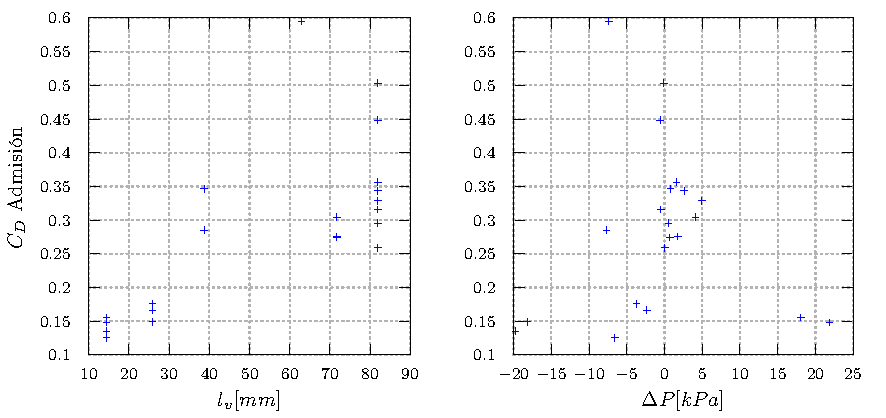
\includegraphics{gnuplot/cd_vs_alzada_adm.pdf}
    \caption{$C_{D}$ del puerto de admisión}\label{fig:cd_admision}
\end{figure}

El máximo coeficiente de descarga vale $C_{D,\max}\simeq 0,6$ para
$l_{v}=62,95 mm$ y $\Delta P\simeq -7,37 KPa$, obteniendo un flujo hacia afuera
del puerto de $122,09 g/seg$.
%
Para este caso se observa un reflujo de gases residuales apenas abre el puerto
de admisión, correspondiendo a un ángulo de cigüeñal de $10^{\circ}$ a $7000$
RPM.

La flujometría correspondiente al último instante de la simulación se muestra en
la Figura~\ref{fig:adm_cd_max}, en la cual las líneas de corriente están
coloreadas según el módulo de la velocidad y las flechas indican el sentido de
flujo.
%
La mayor velocidad del flujo se da en el gas que sale de la cámara,
correspondiente a masa residual atrapada luego del barrido del puerto de escape.


El flujo másico máximo hacia adetro de la cámara ($\Delta P>0$) ocurre para la
misma geometría indicada en la Figura~\ref{fig:adm_cd_max}.
%
Se alcanza $\dot{m}_{\max}\simeq 70 g/seg$ para la cámara que se encuentra más
avanzada en el proceso de admisión y con máxima apertura del puerto con
$l_{v}=81,94 mm$ y $\Delta P=4,95 KPa$ siendo $C_{D}\simeq 0,33$.

\begin{figure}[h]
    \centering
    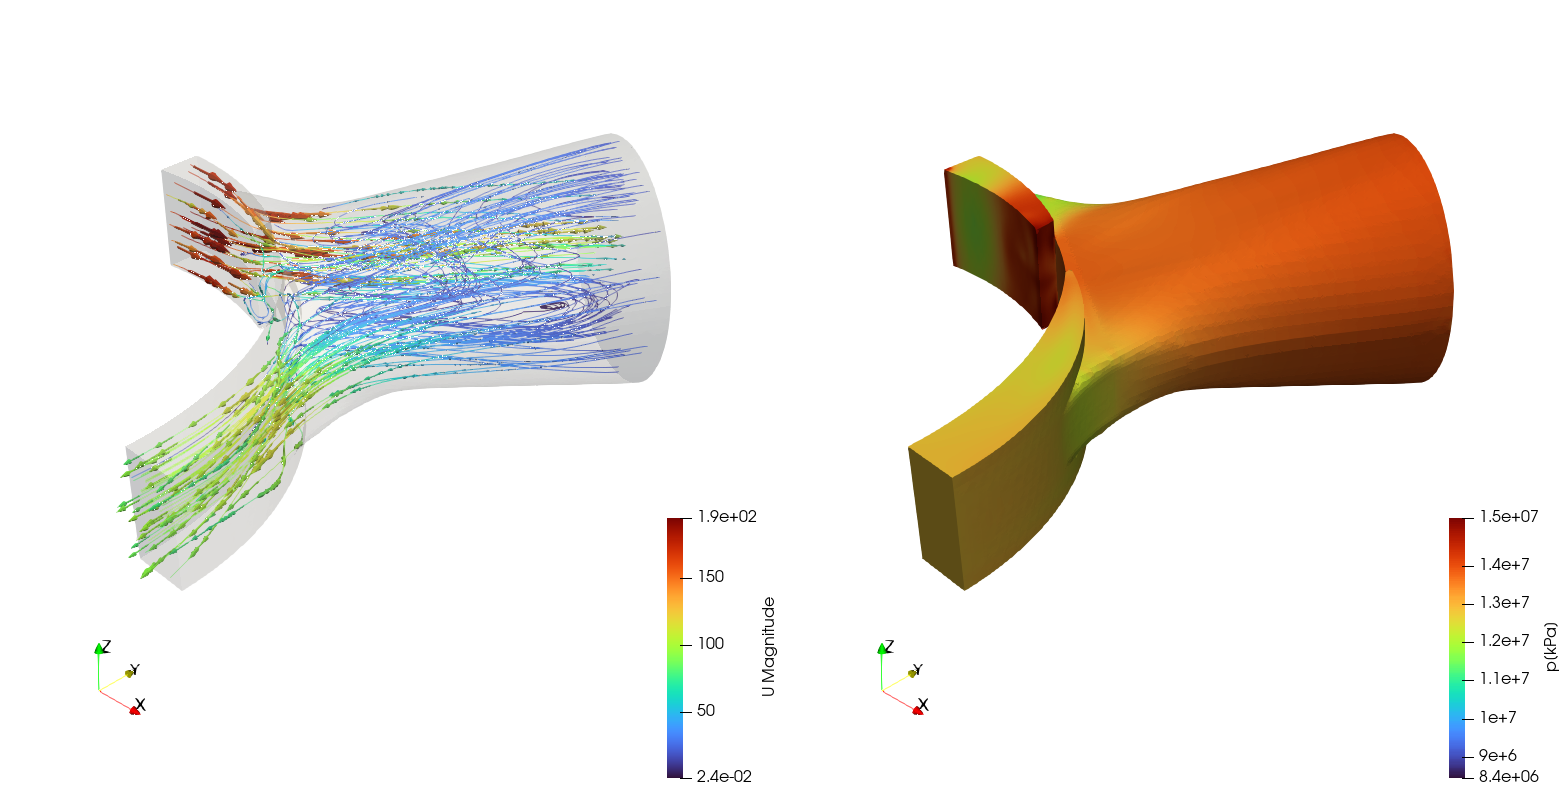
\includegraphics[width=\textwidth]{flujometrias/adm_cd_max.png}
    \caption{Admisión - Máximo $C_{D}$}\label{fig:adm_cd_max}
\end{figure}




\subsection{Puerto de Escape}
%
En la Figura~\ref{fig:mapa_cd_escape} se ilustra el mapa obtenido para el puerto
de escape.
%
La tendencia es similar al puerto de admisión, en la Figura~\ref{fig:cd_escape}
se observa que el coeficiente de descarga es mayor para aperturas mayores del
puerto y menores gradientes de presión ($|\Delta P|\sim 0$).
%
El máximo coeficiente de descarga obtenido vale $C_{D,\max}\simeq 0,58$ y ocurre
para $l_{v}=87,76 mm$, $\Delta P=-10,7 KPa$ con un flujo másico de $145 g/s$
hacia afuera para $440^{\circ}$ a $9000$ RPM, ver Figura~\ref{fig:esc_cd_max}.
%
Por otro lado el máximo caudal másico es $\dot{m}=176,1 g/seg$ y ocurre para
$l_{v}=87,76 mm$ y $\Delta P=-334 KPa$, correspondiendo a $440^{\circ}$ y 7000
RPM, ver Figura~\ref{fig:esc_m_max}.

\begin{figure}[h]
    \centering
    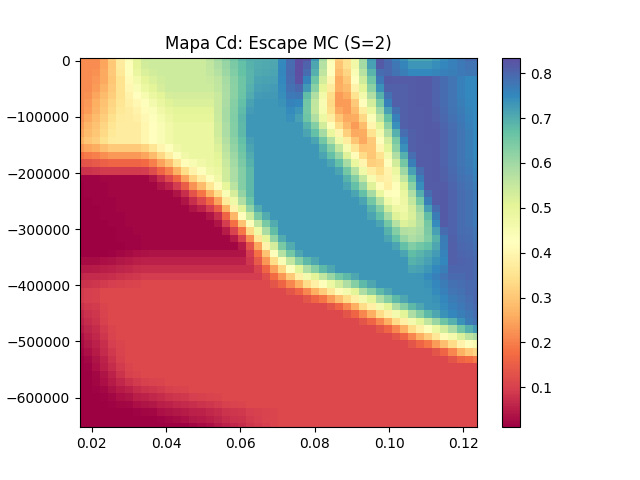
\includegraphics[width=\textwidth]{mapa_cd/mc_s2_mapa_esc.png}
    \caption{Puerto de escape}\label{fig:mapa_cd_escape}
\end{figure}

\begin{figure}[h]
    \centering
    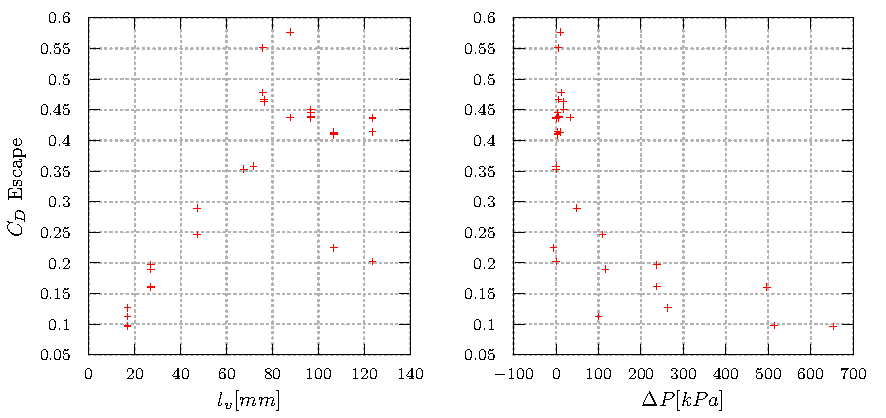
\includegraphics{gnuplot/cd_vs_alzada_esc.pdf}
    \caption{$C_{D}$ del puerto de escape}\label{fig:cd_escape}
\end{figure}


\begin{figure}[h]
    \centering
    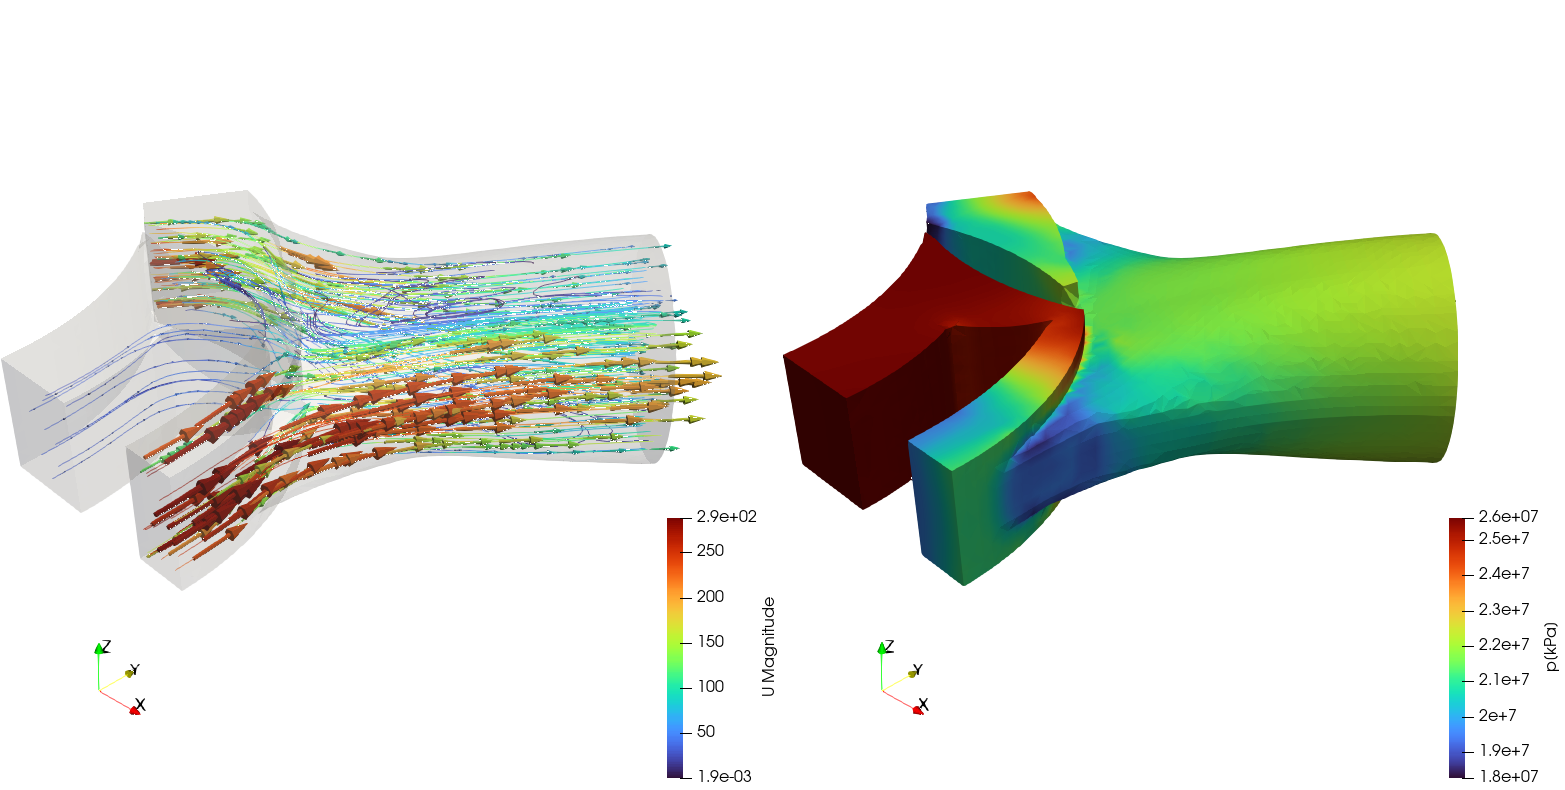
\includegraphics[width=\textwidth]{flujometrias/esc_cd_max.png}
    \caption{Escape - Valor máximo de $C_{D}$}\label{fig:esc_cd_max}
\end{figure}

\begin{figure}[h]
    \centering
    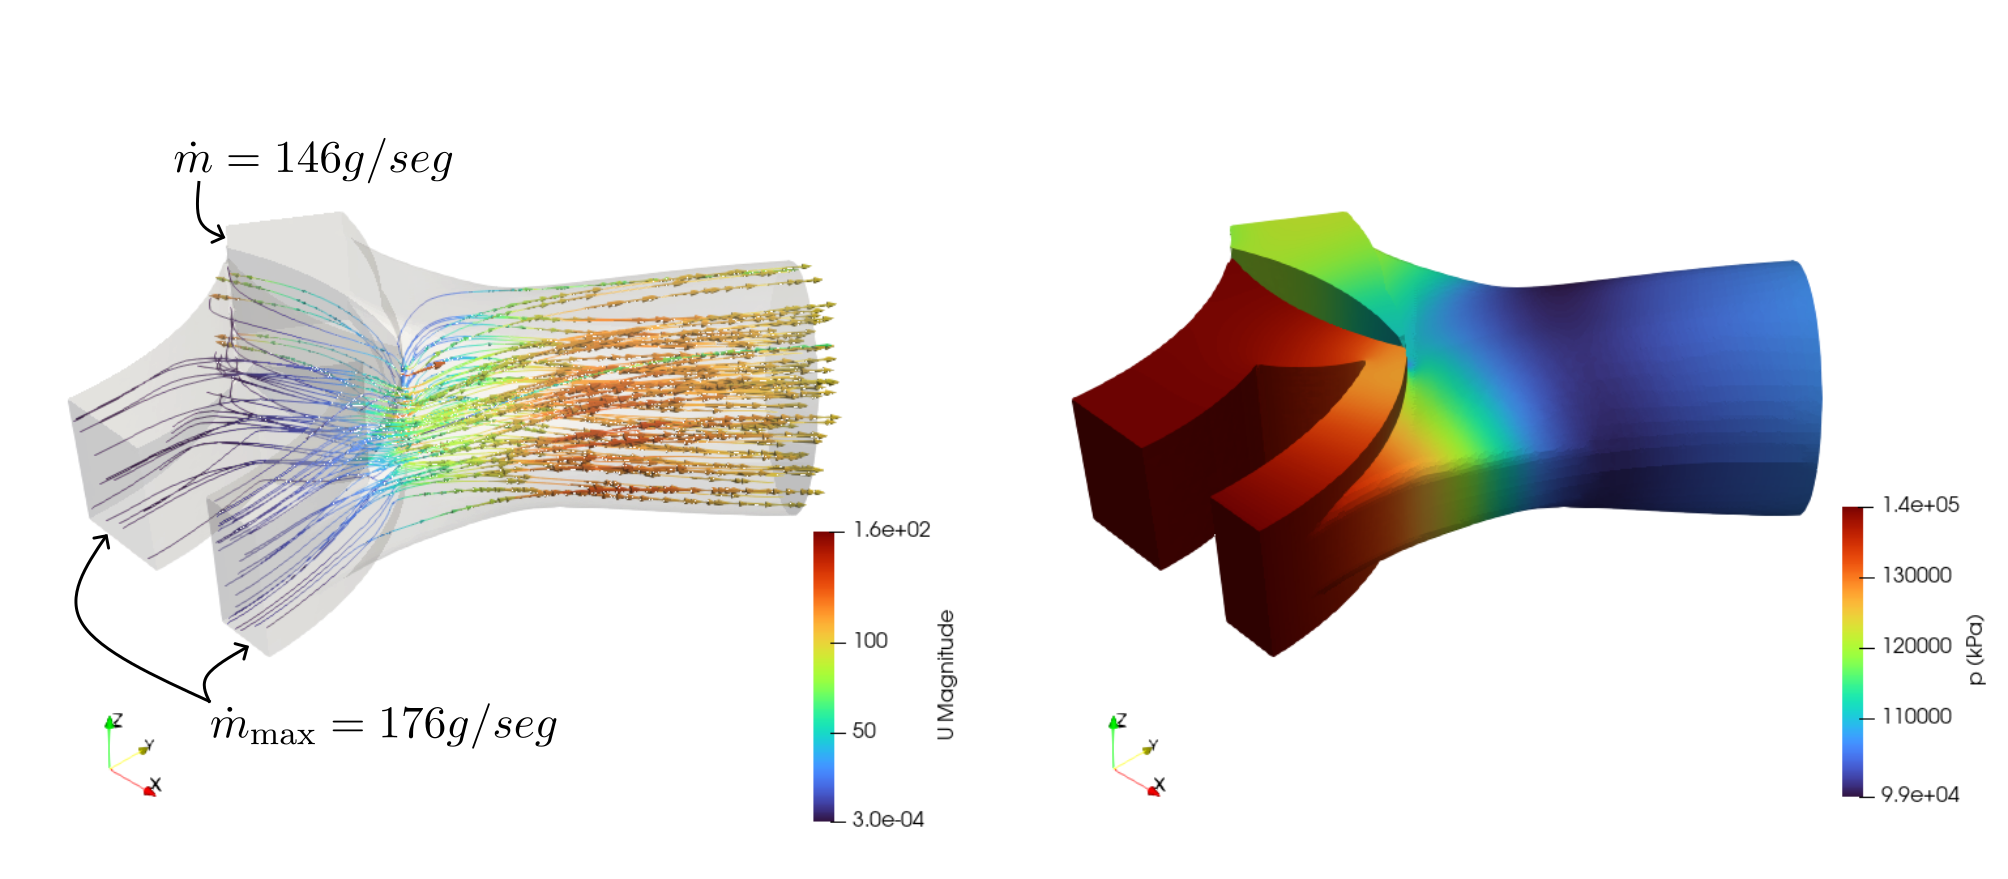
\includegraphics[width=\textwidth]{flujometrias/esc_m_max.png}
    \caption{Escape - Valor máximo de $\dot{m}$}\label{fig:esc_m_max}
\end{figure}
